\chapter{Weryfikacja działania systemu wizyjnego}

Sprawdzenie poprawności działania obu algorytmów miało przebieg trzyetapowy:
\begin{itemize}
	\item model programowy,
	\item symulacja modelu behawioralnego,
	\item uruchomienie algorytmu z warstwą sterującą na dronie.
\end{itemize}

\section{Testy symulacyjne}

Implementacja sprzętowa jest procesem skomplikowanym, w którym łatwo o błąd utrudniający dalszą pracę. Z tego względu istotne jest równoległe przeprowadzanie testów symulacyjnych, które weryfikują poprawność tworzonej logiki. W projekcie testy te realizowano niezależnie dla obu algorytmów śledzących. %TODO 2 to jest dalej niejasne.... - uprościć ! %ODP OK
Za referencję do symulacji obrano uprzednio stworzony model programowy w MATLABie, chociażby ze względu na wykorzystanie tych samych obrazów w celu porównania wyników. 
Moduł symulacyjny stworzony w środowisku Vivado i~języku SystemVerilog nie uwzględniał jedynie części logiki zawartej w \textit{Block Design} -- a więc instancji procesora oraz wejściowego i wyjściowego fragmentu toru wizyjnego. 
Testy procesora nie mają związku z weryfikacją działania algorytmów, a mocno spowalniałyby pracę symulatora. %TODO 2 testy, testowany %ODP OK
Jako zamiennik wejścia informacji wizyjnej, wystarczył zasymulowany komplet sygnałów RGB z informacją o wartości piksela, która została wczytana z pliku tekstowego. 
Plik przechowujący jedną ramkę obrazu, wygenerowano w MATLABie umieszczając każdy kolejny piksel w nowej linii w formacie heksadecymalnym, po dwa znaki na każdą składową R, G i B.

Podstawowej zaletą symulacji jest możliwość podejrzenia propagowanych w układzie sygnałów w oknie wyświetlającym ich przebieg czasowy. 
Jednak ze względu na zwiększający się poziom skomplikowania projektu, z czasem postanowiono uprościć porównanie wybranych wyników symulacji z pracą modelu programowego. 
W kodzie architektury stworzono więc logikę zapisującą do plików określone informacje z pojedynczej iteracji algorytmu. 
By jednak zapis nie był realizowany na każdym zboczu narastającym zegara, potrzebne było określenie sygnałów wyzwalających - -zazwyczaj były to odpowiedniki sygnałów aktywnych powiązanych z~określoną informacją. 
Do analizy stworzono w MATLABie dodatkowy skrypt, który parsował stworzone podczas symulacji pliki, uruchamiał pojedynczy przebieg modelu programowego i~porównywał wyniki, określając liczbę błędów na danym etapie algorytmu dla całej ramki. 
Niektóre dane, z racji ograniczeń związanych ze stałoprzecinkową reprezentacją w architekturze, wymagały zdefiniowania akceptowalnego poziomu tolerancji błędu.
%TODO 2 chyba stałoprzecinkowej - o to Panu chodzi ? %ODP OK


\section{Testy w układzie Zynq}

Symulacje są zbyt kosztownym czasowo narzędziem, dlatego w pewnym momencie należało przejść na testy na urządzeniu PYNQ. 
Proces budowy projektu sprowadza się do stworzenia konfiguracji sprzętowej w Vivado i skompilowania aplikacji uruchamianej na procesorze ARM. 
Docelowo układ SoC może być uruchomiony z poziomu karty SD, jednak ze względu na kwestię praktyczności, pozostano przy połączeniu JTAG. 
Stworzona konfiguracja testowa jest przedstawiona na schemacie \ref{fig:testing_setup}.
Zastosowaniem komputera (PC \#1) jest nie tylko zaprogramowanie układu Zynq poprzez interfejs JTAG, ale i diagnostyczna komunikacja z układem, realizowana poprzez UART. 
Źródłem obrazu wideo może być dowolne urządzenie z możliwością wysłania sygnału \textit{720p} poprzez kabel HDMI. 
W tym wypadku jest to kamera, albo inny komputer -- służący to odtwarzania wcześniej zapisanych materiałów wideo. 
Najważniejszym elementem podczas testów jest wyświetlenie obrazu wyjściowego, z nakreślonymi obszarami detekcji.
\begin{figure}[h]
	\centering
	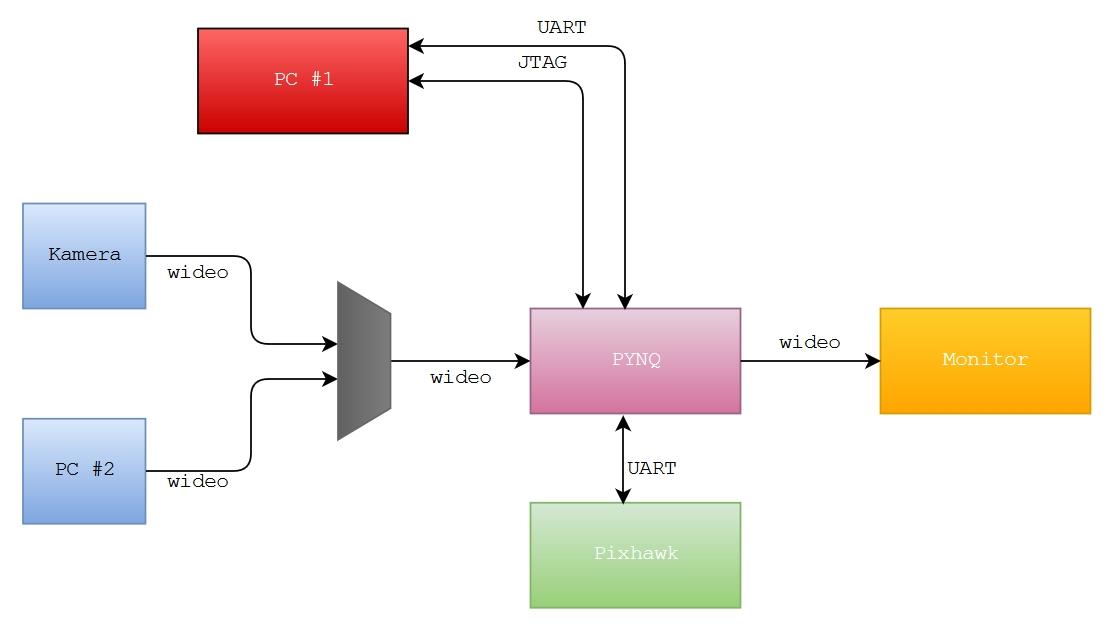
\includegraphics[width=14cm]{6_testing_setup.jpg}
	\caption{Schemat stanowiska testowego}
	\label{fig:testing_setup}
\end{figure}

Test polega na skanowaniu ruchomego obrazu w poszukiwaniu postaci, a następnie śledzeniu znalezionej osoby. 
Analiza jest rozpoczynana w lewym górnym rogu, po czym sukcesywnie przechodzi w linii poziomej do prawej krawędzi, co jest następnie powtarzane dla niższych pozycji \ref{fig:scan_scheme}.
Na przykładowych zrzutach z materiału wideo \ref{fig:scan_screenshot} zaprezentowano proces skanowania obrazu. 
Niebieskimi prostokątami oznaczone są aktualne okna detekcji dla poszczególnych skal. 
Zielone okno to obszar śledzenia algorytmem MeanShift, natomiast czerwonym kolorem oznaczono aktualnie najlepsze okno $128 \times 64$ (przeskalowane ponownie do oryginalnej rozdzielczości).

\begin{figure}[h]
	\centering
	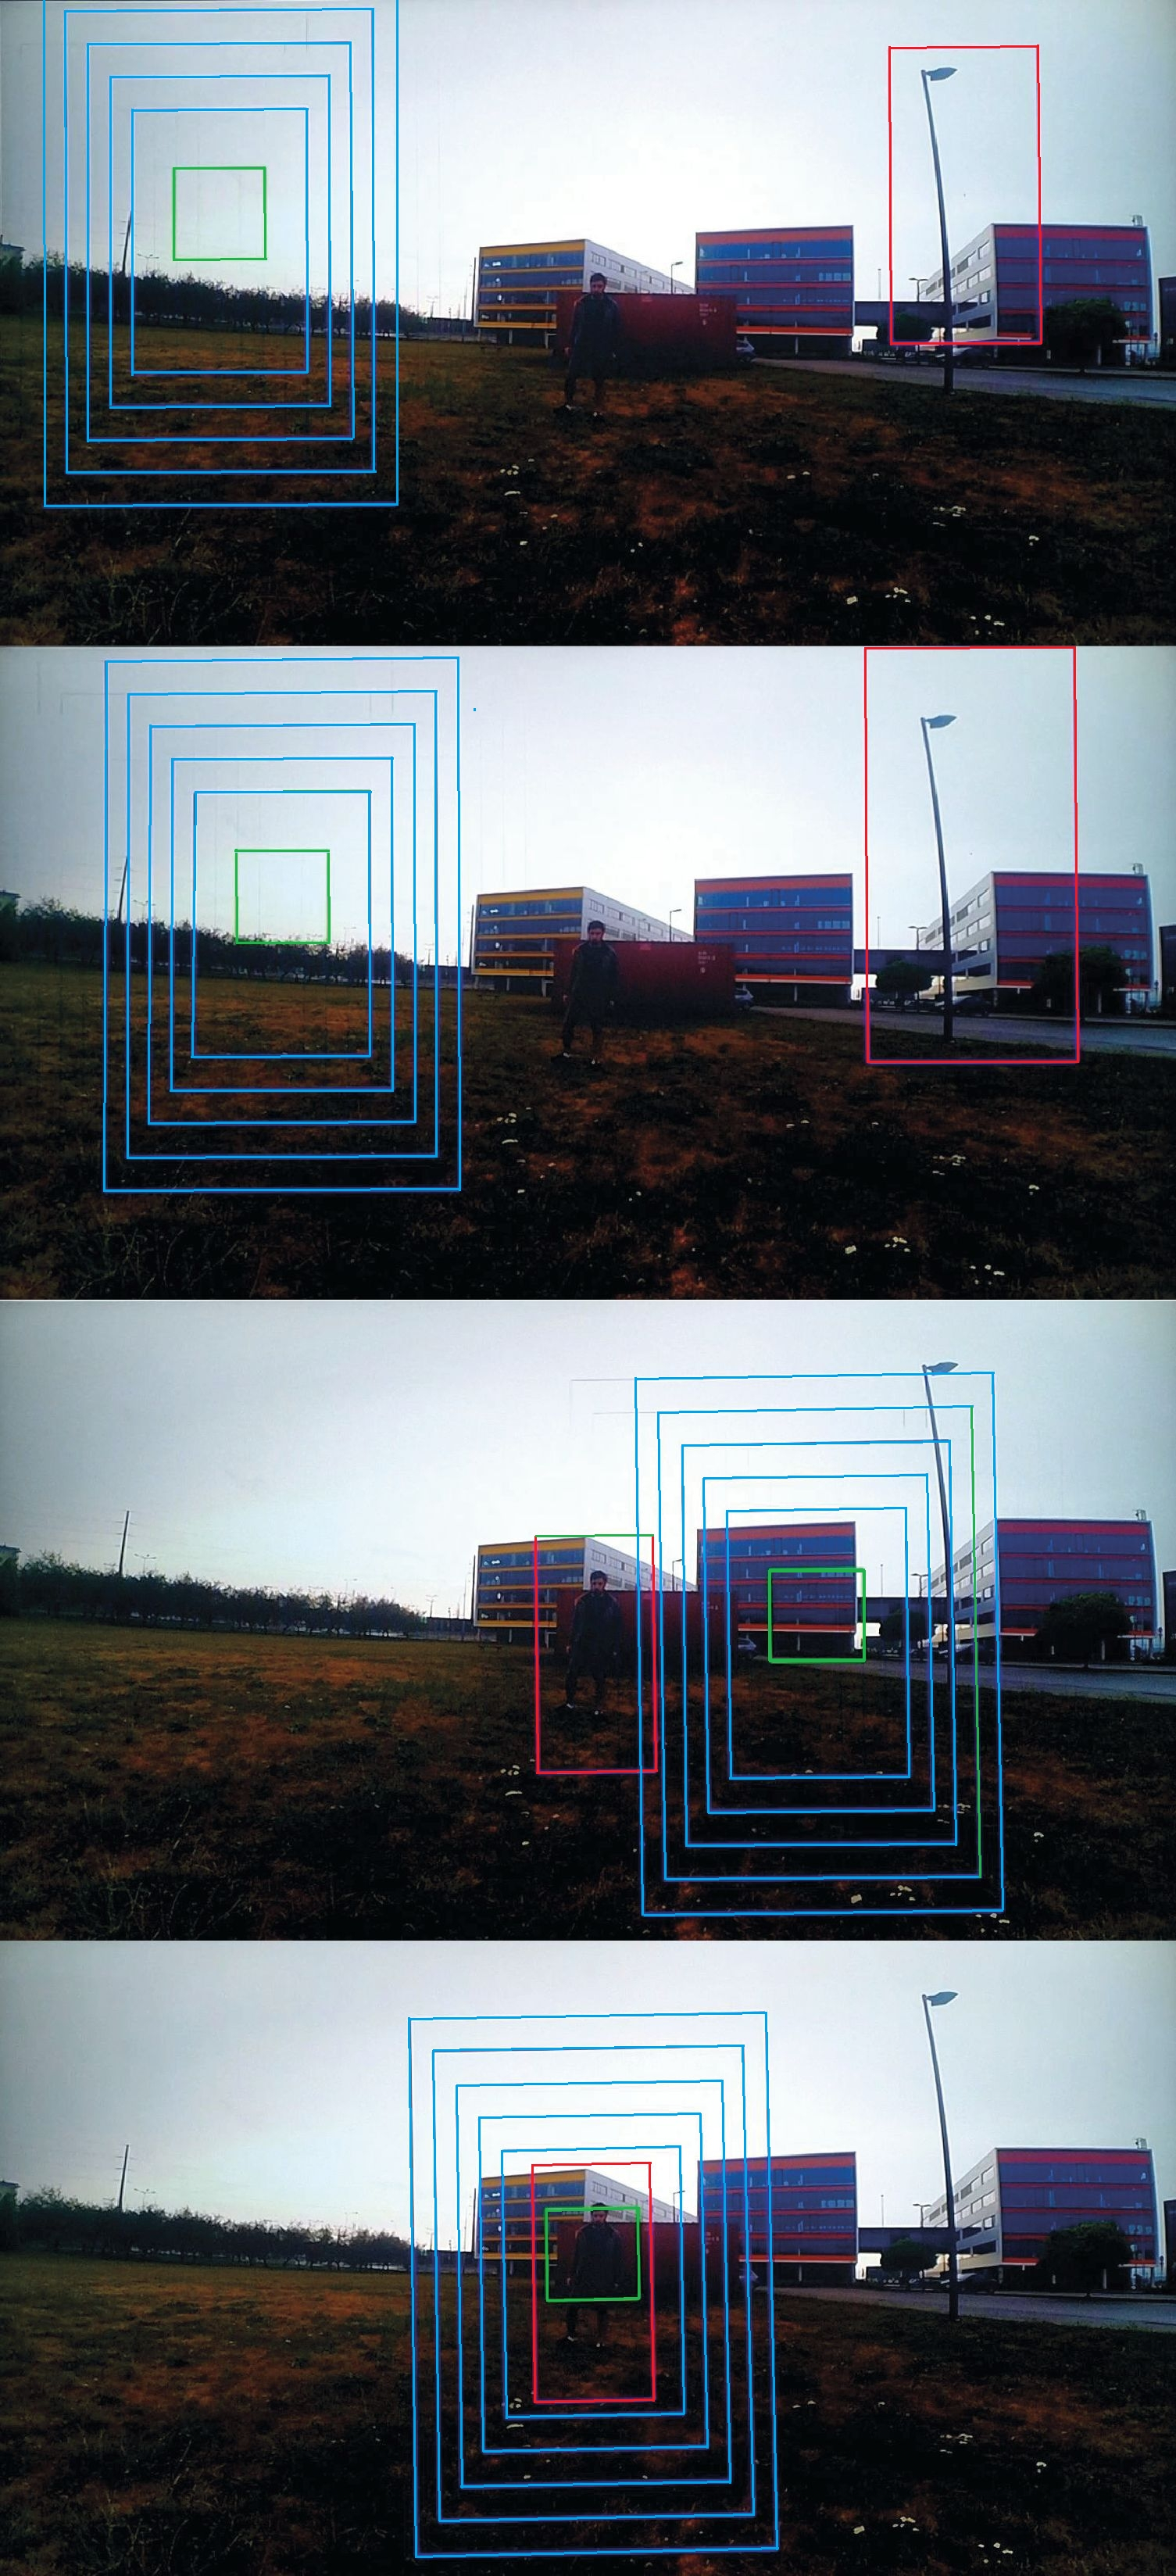
\includegraphics[width=10cm]{6_scan_1.jpg}
	\caption{Proces skanowania} 
	\label{fig:scan_screenshot}
\end{figure}

\begin{figure}[h]
	\centering
	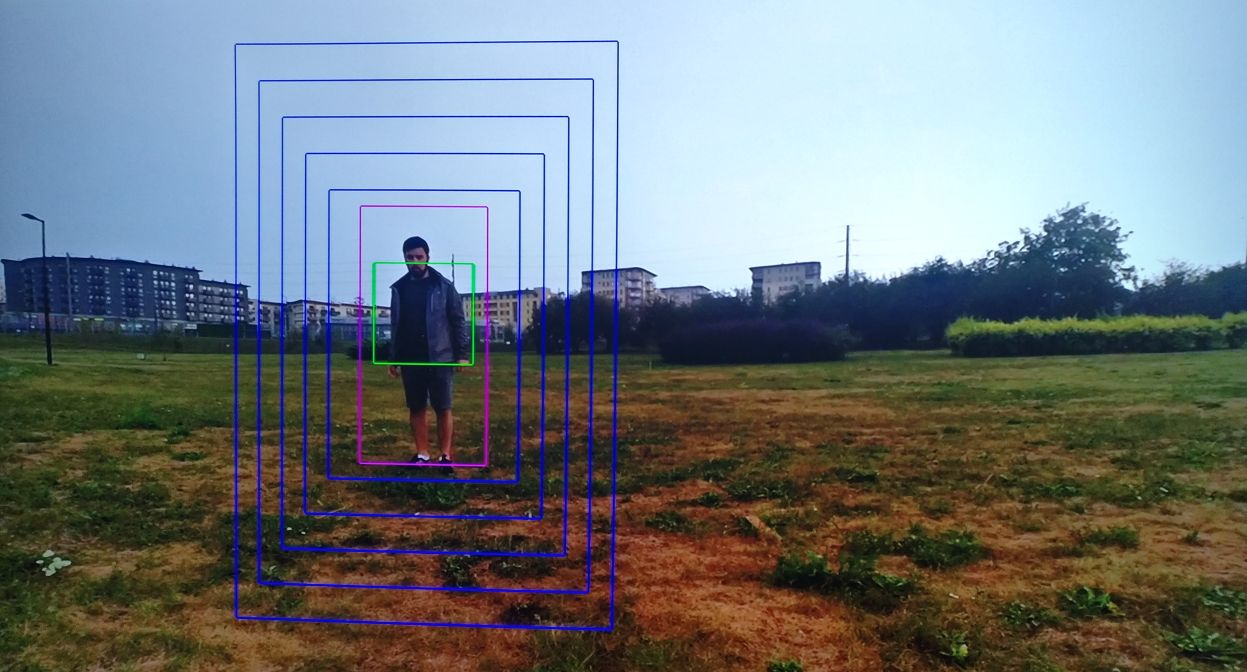
\includegraphics[width=10cm]{6_track_1.jpg}
	\caption{Śledzenie \#1}
	\label{fig:track_1}
\end{figure}

\begin{figure}[h]
	\centering
	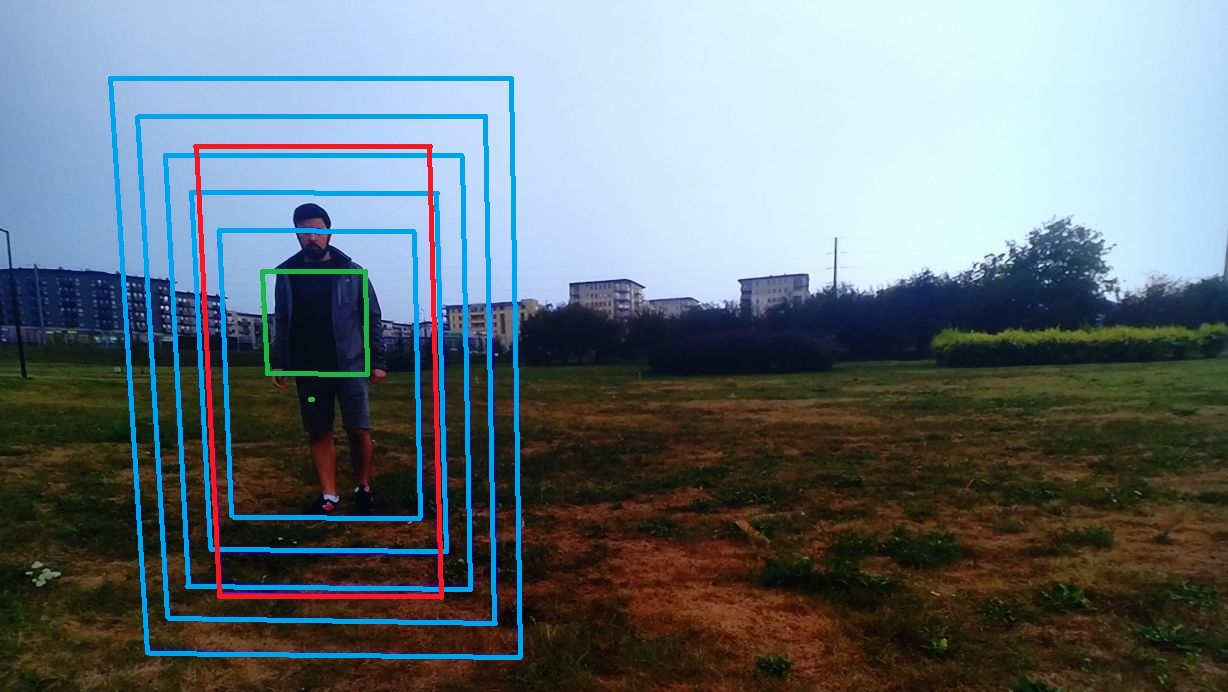
\includegraphics[width=10cm]{6_track_2.jpg}
	\caption{Śledzenie \#2}
	\label{fig:track_1}
\end{figure}

\begin{figure}[h]
	\centering
	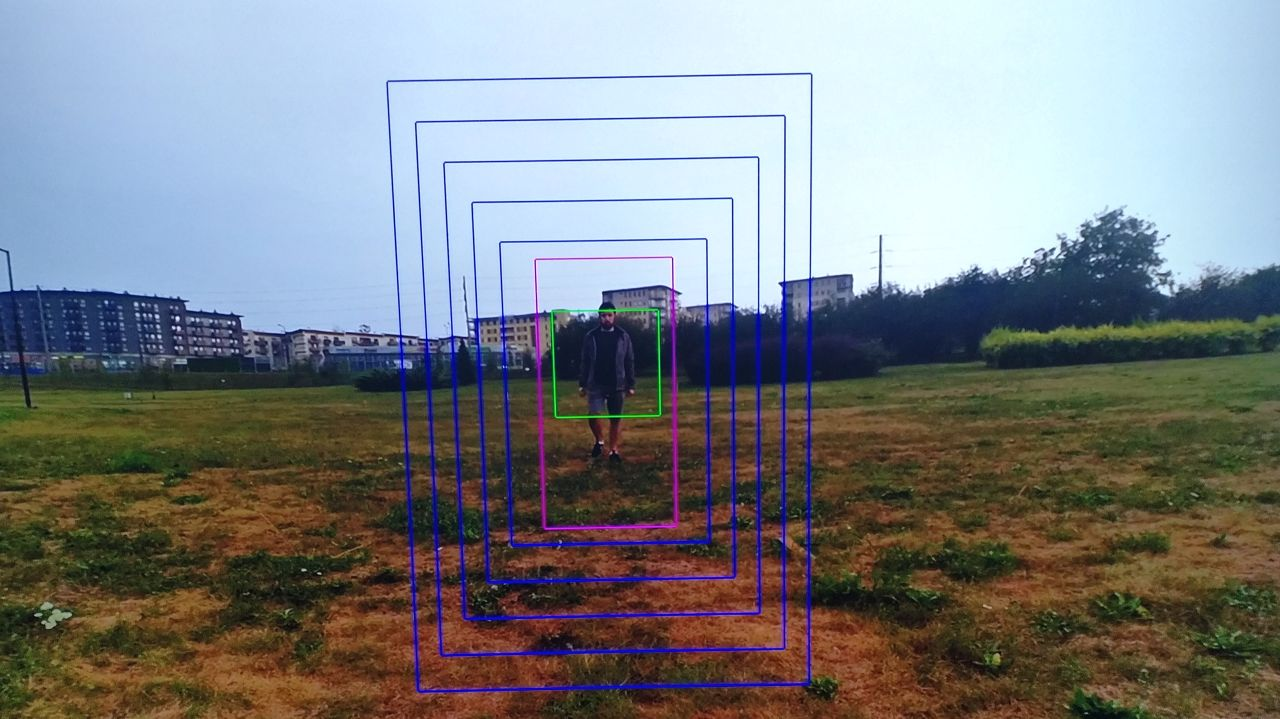
\includegraphics[width=10cm]{6_track_3.jpg}
	\caption{Śledzenie \#3}
	\label{fig:track_1}
\end{figure}

Przebieg testu powinien być jak najbardziej zbliżony do pracy układu podczas lotu, z tego względu do procedury dodano komunikację UART z autopilotem. 
Nadzór nad nią jest sprawowany poprzez dodatkowe połączenie szeregowe łączące układ Zynq z komputerem, który wyświetla w oknie terminala wszystkie istotne komunikaty. 
Przykładowo, raport \ref{tab:log} przedstawia informacje uzyskane w ciągu pierwszych kilkunastu sekund jednego z testów. 
Po otrzymaniu sygnału startu (przełącznik na układzie PYNQ lub na aparaturze radiowej) do autopilota wysyłana jest komenda uzbrojenia (ARM) i startu (TAKEOFF), jednak ze względu na obecność drona w budynku niemożliwe jest określenie pozycji poprzez GPS -- odebrana z autopilota wiadomość COMMAND ACK informuje, że wykonanie komendy TAKEOFF (ID: 22) się nie powiodło (status: 4). 
Podczas testu naziemnego ten komunikat jest jednak ignorowany i rozpoczynany jest proces skanowania. 
Po dłuższej chwili układ wysyła informację o pozytywnym wyniku detekcji, po czym system rozpoczyna zadanie śledzenia. 
Od tego momentu większość komunikatów dotyczy informacji z PL o odległości śledzonego obiektu od wartości zadanej w pionie i poziomie. 
Trzecią wartością jest uśredniony wynik skali z 4 ostatnich detekcji -- wartość przemnożona przez 10 z powodu braku funkcji wyświetlającej liczby zmiennoprzecinkowe. 
Niezależnie od przebiegu pracy systemu wizyjnego mogą pojawiać się wiadomości z~autopilota o~statusie (INFO). 
Test jest przerywany przez użytkownika w momencie zmiany pozycji przełącznika sygnału startu -- oprócz zakończenia pracy algorytmu wysyłana jest wówczas komenda lądowania (LAND).


%TODO 2 No tu jeszzce brakuje testów "polowych" chociaż krótki komentarz, że to działa - tak jak na tym filmie. %ODP OK, niżej


\begin{table}[h]
	\centering\scriptsize 
	
	\begin{tabular}{|p{8cm} |}
		
        \hline
prompt>>ARMING... \\
ARMED! \\
TAKING OFF... \\
Sent TAKEOFF CMD. \\
COMMAND ACK: 22 4 \\
STARTING SEARCH! \\
xDiff: 37        \tab yDiff: 33      \tab| scale: 27 || \\
DATA OK, STARTING FOLLOW! \\
xDiff: 20        \tab yDiff: 20      \tab| scale: 25 || \\
xDiff: 10        \tab yDiff: 20      \tab| scale: 25 || \\
xDiff: 52        \tab yDiff: 38      \tab| scale: 22 || \\
xDiff: 94        \tab yDiff: 8       \tab\tab| scale: 22 || \\
xDiff: 140       \tab yDiff: 12      \tab| scale: 20 || \\
xDiff: 165       \tab yDiff: 30      \tab| scale: 25 || \\
xDiff: 157       \tab yDiff: 22      \tab| scale: 22 || \\
xDiff: 125       \tab yDiff: 40      \tab| scale: 25 || \\
xDiff: 95        \tab yDiff: 35      \tab| scale: 22 || \\
xDiff: 62        \tab yDiff: 26      \tab| scale: 20 || \\
xDiff: 26        \tab yDiff: 28      \tab| scale: 20 || \\
xDiff: 10        \tab yDiff: 28      \tab| scale: 20 || \\
xDiff: -6         \tab\tab yDiff: 28      \tab| scale: 20 || \\
xDiff: -30        \tab yDiff: 36      \tab| scale: 20 || \\
xDiff: -70        \tab yDiff: 28      \tab| scale: 20 || \\
xDiff: -86        \tab yDiff: 20      \tab| scale: 20 || \\
xDiff: -118       \tab yDiff: 28      \tab| scale: 20 || \\
xDiff: -150       \tab yDiff: 12      \tab| scale: 20 || \\
xDiff: -150       \tab yDiff: 12      \tab| scale: 20 || \\
xDiff: -110       \tab yDiff: 20      \tab| scale: 20 || \\
xDiff: -86        \tab yDiff: 20      \tab| scale: 20 || \\
xDiff: -62        \tab yDiff: 28      \tab| scale: 20 || \\
INFO: PreArm: Throttle below Failsafe \\
xDiff: 22        \tab yDiff: 28      \tab| scale: 20 || \\
xDiff: 30        \tab yDiff: 4       \tab\tab| scale: 22 || \\
xDiff: 62        \tab yDiff: 42      \tab| scale: 27 || \\
xDiff: 95        \tab yDiff: 33      \tab| scale: 27 || \\
xDiff: 107       \tab yDiff: 33      \tab| scale: 30 || \\
xDiff: 107       \tab yDiff: 33      \tab| scale: 30 || \\
xDiff: 107       \tab yDiff: 33      \tab| scale: 30 || \\
xDiff: 172       \tab yDiff: 34      \tab| scale: 20 || \\
xDiff: 268       \tab yDiff: 14      \tab| scale: 20 || \\
xDiff: 368       \tab yDiff: 14      \tab| scale: 22 || \\
xDiff: 450       \tab yDiff: 20      \tab| scale: 25 || \\
xDiff: 560       \tab yDiff: 15      \tab| scale: 22 || \\
Sent LAND CMD. \\
COMMAND ACK: 21 0 \\    
\hline 	
	\end{tabular}
	\caption{Przykładowa zawartość terminala ze śledzenia na podstawie gotowego materiału wideo}
	\label{tab:log}
\end{table}

Ostatnim etapem testów było uruchomienie w pełni sprawnego systemu wizyjnego na platformie UAV. W ich trakcie nie tylko zweryfikowano poprawność działania systemu detekcji i~śledzenia, ale również dostosowano parametry regulatora, który poprzez komunikację z autopilotem wpływał na ruch drona.